%%%%%%%%%%%%%%%%%%%%%%%%%%%%%%%%%%%%%%%%%%%%%%%%%%%%%%%%%%%%%%%%%%%%%%%%%%%%%%%%%%%%%%%%%%%%%%%%%%

%% document class
%\documentclass{beamer}
%\documentclass[aspectratio=169]{beamer}
\documentclass{beamer}

%% packages
%% packages

\usepackage{blindtext} % needed for creating dummy text passages
%\usepackage{ngerman} % needed for German default language
\usepackage{amsmath} % needed for command eqref
\usepackage{amsthm}
\usepackage{amssymb} % needed for math fonts
\usepackage[
	colorlinks=true
	,breaklinks
	%,ngerman
	]{hyperref} % needed for creating hyperlinks in the document, the option colorlinks=true gets rid of the awful boxes, breaklinks breaks lonkg links (list of figures), and ngerman sets everything for german as default hyperlinks language
%\usepackage[hyphenbreaks]{breakurl} % ben�tigt f�r das Brechen von URLs in Literaturreferenzen, hyphenbreaks auch bei links, die �ber eine Seite gehen (mit hyphenation).
\usepackage{aliascnt}
\usepackage{xcolor}
\definecolor{c1}{rgb}{0,0,1} % blue
\definecolor{c2}{rgb}{0,0.3,0.9} % light blue
\definecolor{c3}{rgb}{0.3,0,0.9} % red blue
\hypersetup{
    linkcolor={c1}, % internal links
    citecolor={c2}, % citations
    urlcolor={c3} % external links/urls
}
%\usepackage{cite} % needed for cite
\usepackage[square,sort,comma,numbers]{natbib} % needed for cite and abbrvnat bibliography style
\usepackage[nottoc]{tocbibind} % needed for displaying bibliography and other in the table of contents
\usepackage{braket}%braketnotationpackage
\usepackage{graphicx} % needed for \includegraphics 
\usepackage{longtable} % needed for long tables over pages
\usepackage{bigstrut} % needed for the command \bigstrut
\usepackage{enumerate} % needed for some options in enumerate
\usepackage{todonotes} % needed for todos
\usepackage{makeidx} % needed for creating an index
\usepackage{array} % for tables and arrays
\makeindex

\usepackage{caption}%for image captions
\captionsetup[figure]{font=small}

\usepackage{float}%%figures forced wherever

\usepackage{indentfirst}

\usepackage[utf8]{inputenc}
\usepackage[greek,english]{babel}
\usepackage{lmodern}

\usepackage[toc,page]{appendix}

\usepackage{spverbatim}

%% page settings
%% page settings

\usepackage[top=2.5cm, bottom=3.5cm,left=2.5cm,right=2.5cm]{geometry} % needed for page border settings
\parindent=1.5cm % for space of first line of new text block
\sloppy % for writing with hyphenless justification (tries to)
\hyphenation{} % use hyphenation of tolerance parameters, http://www.jr-x.de/publikationen/latex/tipps/zeilenumbruch.html
\hyphenpenalty=10000
\exhyphenpenalty=10000
\usepackage{fancyhdr} % needed for head and foot options

\usepackage{setspace}
\onehalfspacing % or \doublespacing

\allowdisplaybreaks[1]

%% Theme
%\usetheme{Warsaw} % theme for slides
%\usetheme{Frankfurt}
%\usetheme{Madrid}
%\usetheme{Darmstadt}
%\usetheme{Copenhagen}
%\usetheme{Szeged}
%\usetheme{Goettingen}

%% Colors
%\usecolortheme{rose} % color for slides
%\usecolortheme{default}
%\usecolortheme{rose}
%\usecolortheme{seahorse}
%\definecolor{c1}{rgb}{0,0.7,0.6} % some green
%\definecolor{c2}{rgb}{0.9,0.9,0.9} % some gray
%% see http://www.sharelatex.com/learn/Beamer
%\setbeamercolor*{palette primary}{fg=white,bg=c1} % upper part
%\setbeamercolor*{palette secondary}{bg=c2} % left part (background)
%\setbeamercolor*{sidebar left}{fg=white,bg=c1} % left part with links
%\setbeamerfont{section number projected}{ % section numbers
%  family=\rmfamily,
%  series=\bfseries,
%  size=\normalsize
%  }
%\setbeamercolor{section number projected}{bg=c1} % color of section numbers and others (fg: Fontm, bg:Hintergrund)
%\setbeamercolor{item projected}{bg=c1}
%\setbeamercolor{itemize item}{fg=c1}
%\setbeamercolor{author in sidebar}{fg=white}
%\setbeamercolor{footlinecolor}{fg=black,bg=c2}

%% Fonts
%\usefonttheme{professionalfonts} % changes fonts

%% Foot
%\usenavigationsymbolstemplate{} % deafult controls off
%\setbeamertemplate{footline}[frame number] % slide number at the bottom
%\setbeamertemplate{footline}
%{%
%	\leavevmode%
%	\hbox{%
%	\begin{beamercolorbox}[wd=.3\paperwidth,ht=5ex,dp=1.5ex,left,leftskip=2mm]{footlinecolor}%
%		Foot information on the left over several lines
%	\end{beamercolorbox}%
%	\begin{beamercolorbox}[wd=.5\paperwidth,ht=5ex,dp=1.5ex,left,leftskip=2mm]{footlinecolor}%
%		Next foot part
%	\end{beamercolorbox}%
%	\begin{beamercolorbox}[wd=.2\paperwidth,ht=5ex,dp=1.5ex,right,rightskip=2mm]{footlinecolor}%
%		\insertframenumber{} / \inserttotalframenumber%
%	\end{beamercolorbox}%
%	}%
%	\vskip0pt%
%}

%% new commands
%% my macros

%% Text fomats
\newcommand{\tbi}[1]{\textbf{\textit{#1}}}

%% Math fonts
\newcommand{\bbA}{\mathbb{A}}
\newcommand{\bbB}{\mathbb{B}}
\newcommand{\bbC}{\mathbb{C}}
\newcommand{\bbD}{\mathbb{D}}
\newcommand{\bbE}{\mathbb{E}}
\newcommand{\bbF}{\mathbb{F}}
\newcommand{\bbG}{\mathbb{G}}
\newcommand{\bbH}{\mathbb{H}}
\newcommand{\bbI}{\mathbb{I}}
\newcommand{\bbJ}{\mathbb{J}}
\newcommand{\bbK}{\mathbb{K}}
\newcommand{\bbL}{\mathbb{L}}
\newcommand{\bbM}{\mathbb{M}}
\newcommand{\bbN}{\mathbb{N}}
\newcommand{\bbO}{\mathbb{O}}
\newcommand{\bbP}{\mathbb{P}}
\newcommand{\bbQ}{\mathbb{Q}}
\newcommand{\bbR}{\mathbb{R}}
\newcommand{\bbS}{\mathbb{S}}
\newcommand{\bbT}{\mathbb{T}}
\newcommand{\bbU}{\mathbb{U}}
\newcommand{\bbV}{\mathbb{V}}
\newcommand{\bbW}{\mathbb{W}}
\newcommand{\bbX}{\mathbb{X}}
\newcommand{\bbY}{\mathbb{Y}}
\newcommand{\bbZ}{\mathbb{Z}}

%%For theorems and stuff
\newtheorem*{theorem}{Theorem}
\newtheorem{definition}{Definition}
\numberwithin{definition}{section}
\newcommand{\defref}[1]{def \ref{#1}}
\newcommand{\secref}[1]{section \ref{#1}}
\newtheorem{proposition}{Proposition}
\numberwithin{proposition}{chapter}
\newcommand{\propref}[1]{prop \ref{#1}}

\newtheorem*{note}{Note}

%%renewcommands
%\renewcommand{\operatorname}[1]{\tbi{#1}}
\DeclareMathOperator{\Tr}{ \textup{\textbf{Tr}} }
\DeclareMathOperator{\diag}{ diag }
\DeclareMathOperator{\supp}{ \textup{supp}}

%%%%%%%%%%%%%%%%%%%%%%%%%%%%%%%%%%%%%%%%%%%%%%%%%%%%%%%%%%%%%%%%%%%%%%%%%%%%%%%%%%%%%%%%%%%%%%%%%%%

\begin{document}

%%%%%%%%%%%%%%%%%%%%%%%%%%%%%%%%%%%%%%%%%%%%%%%%%%%%%%%%%%%%%%%%%%%%%%%%%%%%%%%%%%%%%%%%%%%%%%%%%%%
%%%%%%%%%%%%%%%%%%%%%%%%%%%%%%%%%%%%%%%%%%%%%%%%%%%%%%%%%%%%%%%%%%%%%%%%%%%%%%%%%%%%%%%%%%%%%%%%%%%
%%%%%%%%%%%%%%%%%%%%%%%%%%%%%%%%%%%%%%%%%%%%%%%%%%%%%%%%%%%%%%%%%%%%%%%%%%%%%%%%%%%%%%%%%%%%%%%%%%%

\author[]{Stefanopoulos Dimitris}
\title{Physical Examples of Quantum Entropies: Properties, Calculations and Programmability}
%\titlegraphic{\includegraphics[width=0.2\textwidth]%{figures/cube}}
\institute{Aristotle's University of Thessaloniki\\Subatomic Physics and Technological Applications}
\date{Thessaloniki, February 17, 2021}
\frame{\titlepage}

%%%%%%%%%%%%%%%%%%%%%%%%%%%%%%%%%%%%%%%%%%%%%%%%%%%%%%%%%%%%%%%%%%%%%%%%%%%%%%%%%%%%%%%%%%%%%%%%%%%

\begin{frame}{Table of contents}
\tableofcontents
%\tableofcontents[hideallsubsections]
\end{frame}

%%%%%%%%%%%%%%%%%%%%%%%%%%%%%%%%%%%%%%%%%%%%%%%%%%%%%%%%%%%%%%%%%%%%%%%%%%%%%%%%%%%%%%%%%%%%%%%%%%%
%%%%%%%%%%%%%%%%%%%%%%%%%%%%%%%%%%%%%%%%%%%%%%%%%%%%%%%%%%%%%%%%%%%%%%%%%%%%%%%%%%%%%%%%%%%%%%%%%%%

\section{Intro}

\subsection{Motivation}

\begin{frame}{Motivation}
\begin{scriptsize}
\begin{itemize}
\item Ill-defined conventions when calculating quantum entropies (for example $0\ln 0\equiv 0$) work operationally but it is not easy to use them when we automate the calculations with programming languages.
\item It is not easy to find analytic calculations of quantum entropies in the literature.
\item Why a physicist might care about quantum entropies? 
\begin{center}	\fbox{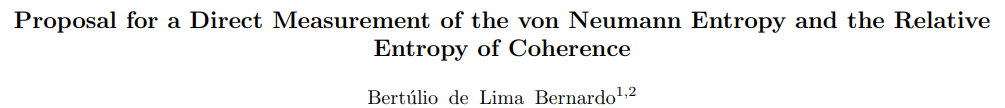
\includegraphics[width=0.85\textwidth]{figures/paperfig}}
\end{center}
\begin{center}
	\fbox{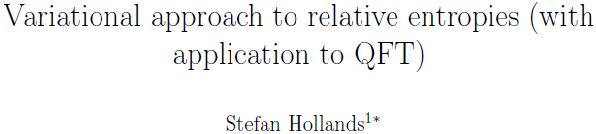
\includegraphics[width=0.6\textwidth]{figures/paperfig2}}
\end{center}
\item Why do we even talk about more than one entropy? Different entropies can describe extra or different phenomena than the common definitions.
\end{itemize}
\end{scriptsize}
\end{frame}

\subsection{Spectral theorem}

\begin{frame}{Functional Calculus}
Common appearance of the spectral theorem:
$$
f(A)=\sum_{i} f\left(\alpha_{i}\right)\left|\phi_{i}\right\rangle\left\langle\phi_{i}\right|
$$
matrix formation:
$$
f(A)=M\left(\begin{array}{cccc}
f\left(\alpha_{1}\right) & 0 & \ldots & 0 \\
0 & f\left(\alpha_{2}\right) & \cdots & 0 \\
& \vdots  & \ddots & \vdots \\
0 & 0 & \cdots & f\left(\alpha_{d}\right)
\end{array}\right) M^{-1}
$$
\begin{alertblock}{Note}
The modal matrix approach of the spectral theorem holds for any simple real-valued measurable function of a $d \times d$  Hermitian matrix.
\end{alertblock}
\end{frame}

\subsection{Quantum Theory}
\begin{frame}{Quantum states and substates}
\begin{scriptsize}
Pure states are ket vectors $\ket{\psi} \in \mathcal{H}$.
The density operator:
$$
\rho = \sum_{i} p_{i}\left|\psi_{i}\right\rangle\left\langle\psi_{i}\right|
$$
with $\Tr \rho=1$,$\rho=\rho^{\dagger}$,$\rho \geq 0$.
\begin{alertblock}{Note}
The randomness of a quantum state expressed via the density matrix has two manifestations.
\end{alertblock}
The reduced substate:
\begin{small}
\begin{align*}
\rho^A &= \Tr_{B}\left( \rho^{AB} \right)=
\sum_{i}\left(I_{A} \otimes\left\langle\left. i\right|_{B}\right) \rho^{AB}\left(I_{A} \otimes|i\rangle_{B}\right)\right) \\  \Tr_B & \left( \sum_{i, j, k, l} p_{ijkl}|i\rangle\left\langle\left. k\right|_{A} \otimes \mid j\right\rangle\left\langle\left. l\right|_{B}\right. \right) = \sum_{i, j, k, l} p_{ijkl} |i\rangle\left\langle\left. k\right|_{A}  \Tr \left(  |j\right\rangle\left\langle l\right|_{B} \right)
\end{align*}
\end{small}
\end{scriptsize}
\end{frame}

\begin{frame}{Entanglement}
\begin{small}
\begin{definition}
A mixed state of a composite system described by a density matrix $\rho$ acting on $\mathcal{H_{A}} \otimes \mathcal{H_{B}}$ is separable if there exist $p_{i} \geq 0,\left\{\rho_{A}^{i}\right\}$ and $\left\{\rho_{B}^{i}\right\}$ for which $\rho^{i}_A \in \mathcal{D}(\mathcal{H_A})$, $\rho^{i}_B \in \mathcal{D}(\mathcal{H_B})$
and
$$
\rho=\sum_{i} p_{i} \rho_{A}^{i} \otimes \rho_{B}^{i}
$$
where $\sum_{i} p_{i}=1$. Otherwise the state is called entangled.
\end{definition} 
\end{small}
\begin{small}
\begin{itemize}
\item The assumption that the physical properties of the system have definite values which exist independent of observation is sometimes known as the assumption of \textit{realism}. 
\item The assumption that a measurement can be performed on system A that does not influence the result of a measurement on system B is sometimes known as the assumption of \textit{locality}.
\end{itemize}
\end{small}
\end{frame}
\begin{frame}{Bell's inequalities}
\begin{scriptsize}
Based on EPR-like states $(|00\rangle+|11\rangle)/\sqrt{2}$ Bell discovered his famous inequalities.
\begin{center}	\fbox{
\includegraphics[width=0.5\textwidth]{figures/paperfig4}}
\end{center}
Assuming a probability distribution of predictive properties $\mathbb{P}$ consistent with \textit{local realism}  we are forced to find $E(\mathbb{P})\leq 2$. However projective measurements lead to $E(\mathbb{P})=2 \sqrt{2}$. Violation of these inequalities is though of as a sufficient criterion for entanglement.
\begin{center}	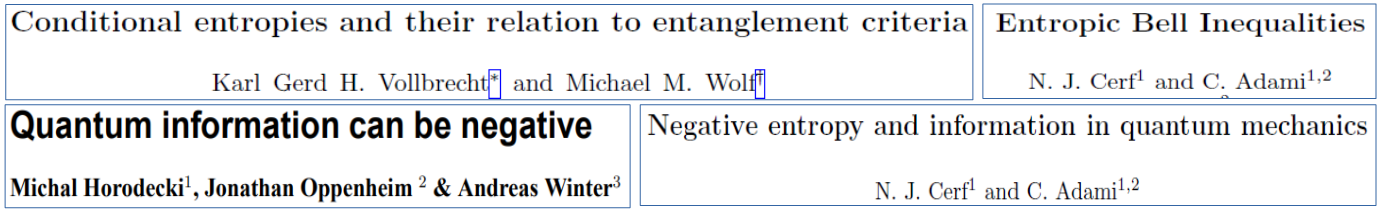
\includegraphics[width=0.9\textwidth]{figures/paperfig8}
\end{center}
\begin{alertblock}{Remark}
\begin{itemize}
\item Negative conditional entropy is necessary condition for entanglement.
\item Positive conditional entropy is a necessary condition for separability.
\end{itemize}
\end{alertblock}
\end{scriptsize}
\end{frame}
\section{Quantum entropies}
\subsection{von Neumann entropy}
\begin{frame}{Basic theory and concepts}
\begin{footnotesize}
\begin{definition}(Von Neumann entropy)The von Neumann entropy of a quantum state $\rho$ is defined as:
\begin{equation*}
S(\rho)\equiv -\Tr(\rho \log \rho).
\end{equation*}
\end{definition}
\begin{definition}(Heuristic von Neumann entropy)For a density matrix $\rho \in \mathcal{D}(\mathcal{H})$ the heuristic form of the von Neumann entropy is defined as:
\begin{equation*}
S(\rho)=-\Tr(F(\rho))
\end{equation*}
in which F is the function $F: [0,1] \rightarrow \mathbb{R}$: 
\begin{equation*}
F(x)=\lim_{\epsilon \to x}(\epsilon \log \epsilon)
\end{equation*}
\end{definition}
For non-symbolic programming:
\begin{equation*}
F(x)= 
 \begin{cases} 
      0 & x=0 \\
      x \log x & x > 0 
\end{cases}
\end{equation*}
\end{footnotesize}
\end{frame}

\begin{frame}{Example-1}
\begin{scriptsize}
A statistical mixture of $N$ orthogonal(mutually exclusive) pure states.
\begin{equation*}
\rho = \sum_{i=0}^{N-1}\rho_{i}\ket{i}\bra{i}= \diag  (\rho_{0},\rho_{1},..,\rho_{N-2},\rho_{N-1})
\end{equation*}
\begin{equation*}
S(\rho) = -\Tr \left[ \diag \big( F(\rho_{0}),F(\rho_{1}),..,F(\rho_{N-2}),F(\rho_{N-1})
 \big) \right]= -\sum_{i=0}^{N-1}\rho_{i} \log \rho_{i} 
\end{equation*}
For a fixed temperature gas at a $T=1 / k_{B} \beta$ in a canonical ensemble model has a density operator:
\begin{equation*}
\rho_{CE}=\frac{\exp (-\beta \hat{H})}{Z}
\end{equation*}
with $\beta$ being a free parameter, $\hat{H}$ and  $\epsilon_{n}$ denotes the Hamiltonian and its eigenvalues and $Z$ the quantum partition function:
\begin{equation*}
Z=\Tr\left(\mathrm{e}^{-\beta \hat{H}}\right)=\sum_{i} \mathrm{e}^{-\beta \epsilon_{i}}
\end{equation*}
based on the condition $\Tr(\rho)=1$. Thus:
\begin{equation*}
\rho_{i}= e^{-\beta \epsilon_{i}}/Z
\end{equation*}
\end{scriptsize}
\end{frame}

\begin{frame}{Conditional von Neumann entropy}
\begin{alertblock}{Note}
Definitions of classical probability theory can not be trivially used for non-commutative algebras.
\end{alertblock}
\begin{definition}(Conditional von Neumann Entropy)The quantum analog of the conditional entropy is defined as:
\begin{equation*}
S(A \mid B) = S(A B)-S(B)
\end{equation*}
Where $S(A B)=S(\rho^{A B})$ and
$S(B)= S\left(\Tr_{A} \rho^{A B}\right)$.
\end{definition}
\end{frame}

\begin{frame}{Example-II}
\begin{scriptsize}
\begin{center}	\fbox{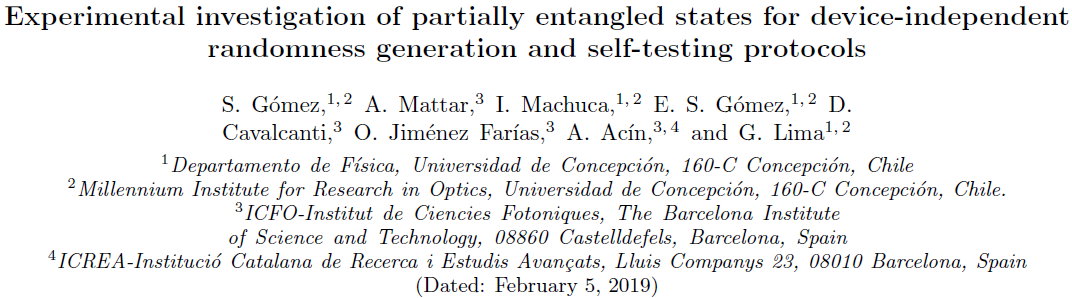
\includegraphics[width=0.8\textwidth]{figures/paperfig9}}
\end{center}
\begin{equation*}
|\psi(\theta)\rangle=\cos \theta|00\rangle+\sin \theta |11\rangle, \quad 0< \theta< \pi /2
\end{equation*}
Its density matrix:
\begin{equation*}
\sigma^{AB}(\theta)=\left(
\begin{array}{cccc}
 \cos ^2 \theta & 0 & 0 & \cos \theta \sin \theta \\
 0 & 0 & 0 & 0 \\
 0 & 0 & 0 & 0 \\
 \cos \theta \sin \theta & 0 & 0 & \sin ^2 \theta  \\
\end{array}
\right)
\end{equation*}
\end{scriptsize}
\end{frame}

\begin{frame}{Example-II}
\begin{scriptsize}
\begin{equation*}
\lambda_1=1,\:  \lambda_2=0,\:  \lambda_3=0,\:  \lambda_4=0, 
\end{equation*}
\begin{equation*}
v_1=\left(
\begin{array}{c}
 \cot \theta \\
 0\\
 0\\
 1 \\
\end{array}
\right),
\:  v_2=\left(
\begin{array}{c}
 -\tan \theta \\
 0\\
 0\\
 1 \\
\end{array}
\right),
\:  v_3= \left(
\begin{array}{c}
 0 \\
 0\\
 1\\
 0 \\
\end{array}
\right),\:  v_4= 
\left(
\begin{array}{c}
 0 \\
 1\\
 0\\
 0 \\
\end{array}
\right)
\end{equation*}
Hence the modal matrix is:
\begin{equation*}
M=\left(
\begin{array}{cccc}
 \cot \theta  & -\tan \theta  & 0 & 0 \\
 0 & 0 & 0 & 1 \\
 0 & 0 & 1 & 0 \\
 1 & 1 & 0 & 0 \\
\end{array}
\right)
\end{equation*}
which gives:
\begin{equation*}
det(M)=-(\cos \theta \sin \theta )^{-1}.
\end{equation*}
As a result:
\begin{equation*}
M^{-1}=
\left(
\begin{array}{cccc}
  \cos  \theta  \sin \theta  & 0 & 0 &  \sin ^2 \theta  \\
 - \cos   \theta  \sin  \theta  & 0 & 0 & \cos ^2 \theta  \\
 0 & 0 & 1 & 0 \\
 0 & 1 & 0 & 0 \\
\end{array}
\right)
\end{equation*}
\end{scriptsize}
\end{frame}

\begin{frame}{Example-II}
\begin{scriptsize}
So we have decomposed $\rho$ as:
\begin{equation*}
\sigma^{AB}=MDM^{-1}
\end{equation*}
in which $D=\diag(\lambda_1,\lambda_2,\lambda_3,\lambda_4)$.
\begin{align}
S(\sigma^{AB}) &= -\Tr(F(\sigma^{AB})) \nonumber \\[0.5em]
&= -\Tr (F(MDM^{-1})) \nonumber \\[0.5em]
&=-\Tr \Bigg[
M
\left( \begin{array}{cccc}
 F(1) & 0 & 0 & 0 \\
 0 & F(0) & 0 & 0 \\
 0 & 0 & F(0) & 0 \\
 0 & 0 & 0 & F(0) \\
\end{array}
\right)
M^{-1}
\Bigg]
\nonumber\\[0.5em]
&=0 \nonumber .
\end{align}

The result is expected since $\sigma^{AB}$ is a pure state.
\begin{alertblock}{Remark}
It can be generally proven that pure states have zero von  Neumann entropy, using $\rho=\rho^2$.
\end{alertblock}
\end{scriptsize}
\end{frame}

\begin{frame}{Example-II}
\begin{scriptsize}
Let's trace out the second qubit using braket notation and the linearity of the partial trace operator: 
\begin{align}
\sigma^A &= \Tr_B (\sigma^{AB}) \nonumber \\[0.5em]
&= \Tr_B \big( \cos^2 \theta \ket{00} \bra{00}+ \cos \theta \sin\theta \ket{00} \bra{11} + \cos \theta \sin \theta \ket{11} \bra{00} + \sin^2 \theta \ket{11} \bra{11} \big) \nonumber \\[0.5em]
&= \Tr_B \big(\cos^2 \theta \ket{0} \bra{0} \otimes \ket{0} \bra{0} + \cos \theta \sin\theta \ket{0} \bra{1} \otimes \ket{0} \bra{1} \nonumber \\[0.5em] &+ \cos \theta \sin\theta \ket{1} \bra{0} \otimes \ket{1} \bra{0} +\sin^2 \theta \ket{1} \bra{1} \otimes \ket{1} \bra{1} 
\big) \nonumber \\[0.5em]
&=
\cos^2 \theta \ket{0} \bra{0} \Tr (\ket{0} \bra{0}) + \cos \theta \sin \theta \ket{0} \bra{1} \Tr ( \ket{0} \bra{1}) \nonumber \\[0.5em] &+ \cos \theta \sin\theta \ket{1} \bra{0} \Tr ( \ket{1} \bra{0} ) + \sin^2 \theta \ket{1} \bra{1} \Tr( \ket{1} \bra{1} )
\nonumber \\[0.5em]
&= \cos^2 \theta \ket{0} \bra{0}
+\sin^2 \theta \ket{1} \bra{1}
\nonumber \\[0.5em] &=
\left( \begin{array}{cccc}
 \cos^2 \theta & 0  \\
 0 & \sin^2 \theta  \\
\end{array}
\right). \nonumber
\end{align}
\end{scriptsize}
\end{frame}

\begin{frame}{Example-II}
\begin{scriptsize}
We see that the reduced density operator is diagonal. Hence, we don't need to decompose the matrix further. Let's calculate:
\begin{align}
S(B \mid A)_{\sigma}&=S(\sigma^{AB})-S(\sigma^A)
\nonumber \\[0.5em] &=0-S(\sigma^A) \nonumber \\[0.5em]
&=-S(\sigma^A) \nonumber \\[0.5em]
&=\Tr[F(\sigma^{A})] \nonumber \\[0.5em]
&= \Tr \Big[
\left( \begin{array}{cccc}
 F(\cos^2 \theta) & 0  \\
 0 & F(\sin^2 \theta)  \\
\end{array}
\right)
\Big]
\nonumber \\[0.5em]
&= 
2 \sin ^2 \theta  \log (\sin \theta )+2 \cos ^2 \theta  \log (\cos \theta ) \nonumber
\end{align}
\end{scriptsize}
\end{frame}

\begin{frame}{Example-II}
\begin{scriptsize}
This result demonstrates the general property of the quantum conditional entropy that pure entangled states have negative values. It is actually easy to see from the following plot that at the limits of $\theta \rightarrow 0$ and $
\theta \rightarrow \pi /2$ the measure goes to 0.
\begin{center}
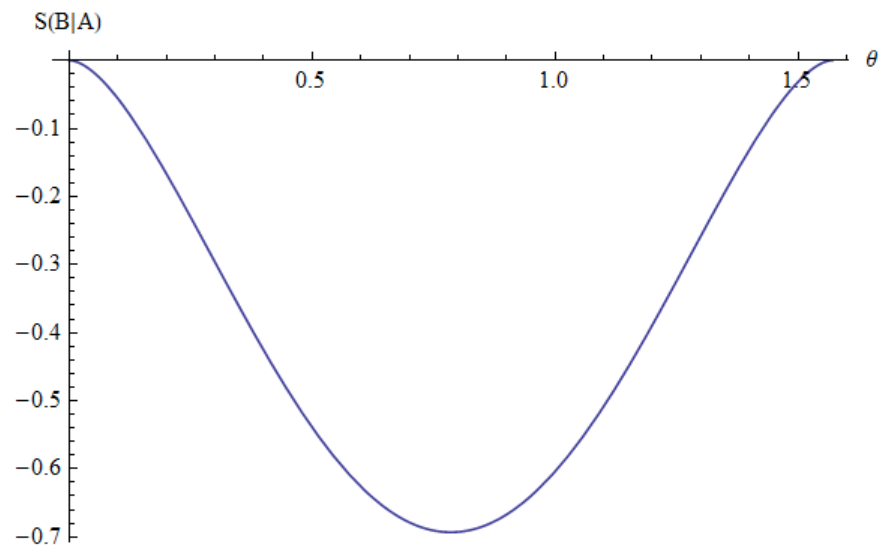
\includegraphics[width=0.7\textwidth]{figures/cond_ent_plot.png}\label{fig1}
\end{center}
We can easily see that the minimum is close to $-\log2$. This is not an accident since is common among the so called maximally entangled states. In particular, $\theta= \pi /4$ will give the maximal entanglement.
\end{scriptsize}
\end{frame}

\begin{frame}{Example-III(Werner states)}
\begin{scriptsize}
\begin{center}
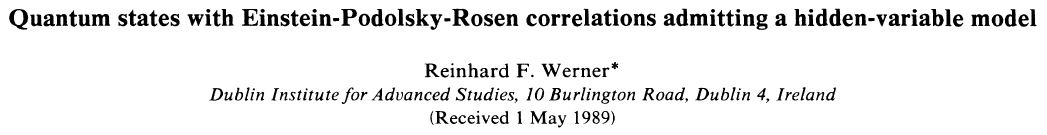
\includegraphics[width=0.9\textwidth]{figures/paperfig10.png}
\end{center}
\begin{center}
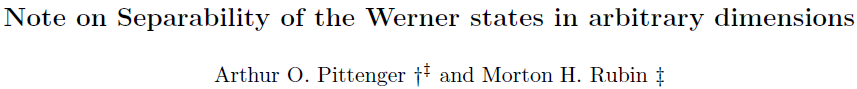
\includegraphics[width=0.7\textwidth]{figures/paperfig11.png}
\end{center}
\begin{equation*}
W^{\left[d^{n}\right]}(s)=(1-s) \frac{1}{d^{n}} I+s|\Psi\rangle\langle\Psi|
\label{wernerstate}
\end{equation*}
where $s$ is a free parameter, $d$ is the dimension of the qudits, $n$ is the number of qudits, $\ket{\Psi}$ is an  entangled state and $I$ is the identity matrix for the composed Hilbert space. It is proven that the state   $W^{\left[d^{n}\right]}(s)$ is fully separable if and only if $s \leq\left(1+d^{n-1}\right)^{-1}$.
We take the simplest case of $d=2$, $n=2$ and $\ket{\Psi}=(\ket{00}+\ket{11})/\sqrt{2}$ as prescribed.
\end{scriptsize} 
\end{frame}

\begin{frame}{Example-III(Werner states)}
\begin{scriptsize}
This state is separable iff $s \leq 1/3$:
\begin{equation*}
W=\left( \begin{array}{cccc}
 (1+s)/4 & 0 & 0 & s/2 \\
 0 & (1-s)/4 & 0 & 0 \\
 0 & 0 & (1-s)/4 & 0 \\
 s/2 & 0 & 0 & (1+s)/4 \\
\end{array}
\right)
\end{equation*}
With
\begin{equation*}
W^A=
\left( \begin{array}{cccc}
 1/2 & 0  \\
 0 & 1/2 \\
\end{array}
\right)
\end{equation*}
\begin{align*}
S(B|A)_{W}&=S(AB)-S(A)
\nonumber \\[0.5em] &= S(W)-S(W^A)
\nonumber \\[0.5em] &= 
\frac{3}{4} (s-1) \log \left(\frac{1-s}{4}\right)-\frac{1}{4} (3 s+1) \log \left(\frac{1}{4} (3 s+1)\right)-\log (2)
\end{align*}
\end{scriptsize}
\end{frame}

\begin{frame}
\begin{center}
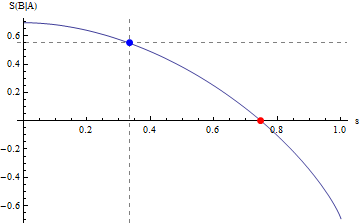
\includegraphics[scale=0.6]{figures/conditional_vonNeumann_Werner.png}\label{fig2}
\end{center}
\begin{scriptsize}
The blue point $B$ has the coordinates $(1/3,0.549306)$ and the red point $R(0.747614,0)$ which was found via numerical methods. The diagram clearly illustrates that the state $W$ while entangled($s\geq 1/3 $) has positive quantum conditional entropy, a fact emphasized by many sources. This particular example becomes negative for $s  \gtrsim 0.747614$.
\end{scriptsize}
\end{frame}

\subsection{Other entropies}
\begin{frame}{Renyi entropy}
\begin{scriptsize}
\begin{definition}(Heuristic quantum Renyi entropy)For a density matrix $\rho \in \mathcal{D}(\mathcal{H})$ the heuristic form of the quantum Renyi entropy is defined as:
\begin{equation*}
R(\alpha ; \rho)= \frac{1}{1-\alpha} \log \Tr \left(r(\alpha;\rho)\right), \alpha \in(0,1) \cup(1, \infty)
\end{equation*}
in which $r$ is the function $r:[0,1] \rightarrow \mathbb{R^{+}}$: $r(\alpha;x)=x^{\alpha}$.
\end{definition}
\begin{alertblock}{Remark}
It is proven that: $\lim _{\alpha \rightarrow 1} R(\alpha;\rho)=S(\rho)$. For $\alpha \to 0$ and $\alpha \to \infty$ the Renyi entropy converges to the Hartley entropy and the Min entropy respectively.
\end{alertblock}
\begin{definition}(Quantum Conditional Renyi Entropy)The conditional form of the quantum Renyi entropy, for a density matrix $\rho \in \mathcal{D}(\mathcal{H})$ is defined as:
\begin{equation*}
R(\alpha;A \mid B)=R(\alpha;\rho^{AB})-R(\alpha;\rho^B)
\end{equation*}
\end{definition}
\end{scriptsize}
\end{frame}

\begin{frame}{Tsallis entropy}
\begin{scriptsize}
\begin{definition}(Heuristic quantum Tsallis entropy)For a density matrix $\rho \in \mathcal{D}(\mathcal{H})$ the heuristic form of the quantum Tsallis entropy is defined as:
\begin{equation*}
T(q ; \rho)= \frac{1}{1-q}\left(\Tr \left[t(q;\rho)\right]-1\right), q \in(0,1) \cup(1, \infty)
\end{equation*}
in which $t$ is the function $t:[0,1] \rightarrow \mathbb{R^{+}}$: $t(q;x)=x^{q}$.
\end{definition}
\begin{alertblock}{Remark}
It can be proved that: $S(\rho)=\lim _{q \rightarrow 1} T(q;\rho)$. For $q \to 0$ and $q \to \infty$ the Tsallis entropy converges to $rank(\rho)-1$ and 0 respectively.
\end{alertblock}
\begin{definition}(Quantum Conditional Tsallis Entropy)The conditional form of the quantum Tsallis entropy,for a density matrix $\rho \in \mathcal{D}(\mathcal{H})$ is defined as:
\begin{equation*}
T(q;A \mid B)=\frac{T(q;\rho^{AB})-T(q;\rho^B)}{1+(1-q) T(q;\rho^{B})}
\end{equation*}
\end{definition}
\end{scriptsize}
\end{frame}

\begin{frame}{Example-IV $\left(\rho(s) = s \ket{0} \bra{0} + (1-s) \ket{1} \bra{1}\right)$}
\begin{scriptsize}
$
R(\alpha;\rho(s))=
\log \left[ s^{\alpha }+(1-s)^{\alpha } \right]/(1-\alpha)
$
\begin{center}
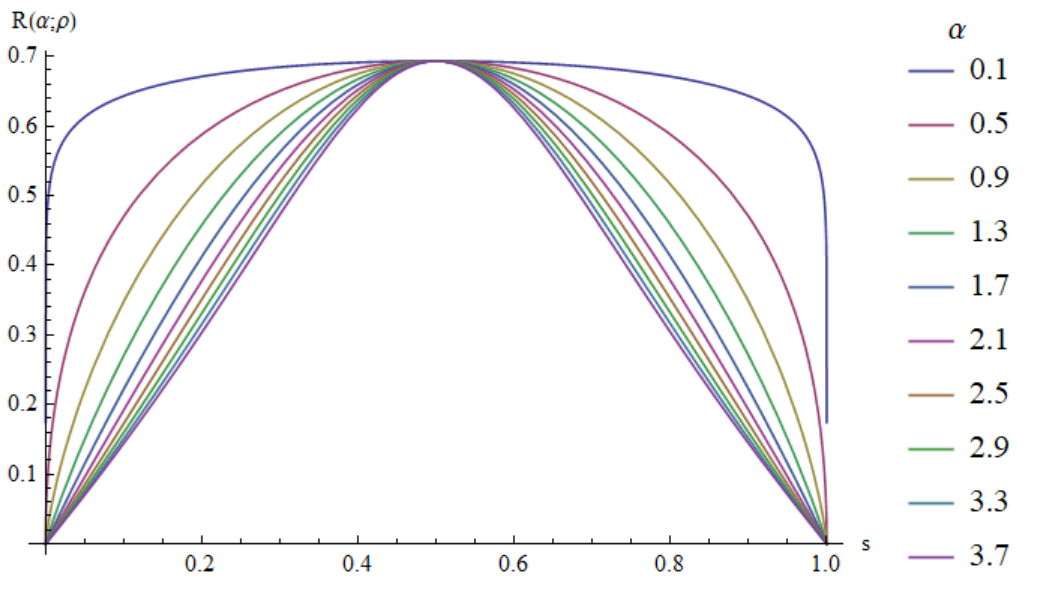
\includegraphics[scale=0.45]{figures/renyi_ent_plot.png}
\end{center}
for $s=0.5$ Renyi entropy takes the value $\log2$ independent of $\alpha$.
\end{scriptsize}
\end{frame}

\begin{frame}{Example-IV $\left(\rho(s) = s \ket{0} \bra{0} + (1-s) \ket{1} \bra{1}\right)$}
\begin{scriptsize}
\begin{equation*}
T(q;\rho(s))=
\left[ s^{q }+(1-s)^{q }-1 \right]/(1-q)
\end{equation*}
\begin{center}
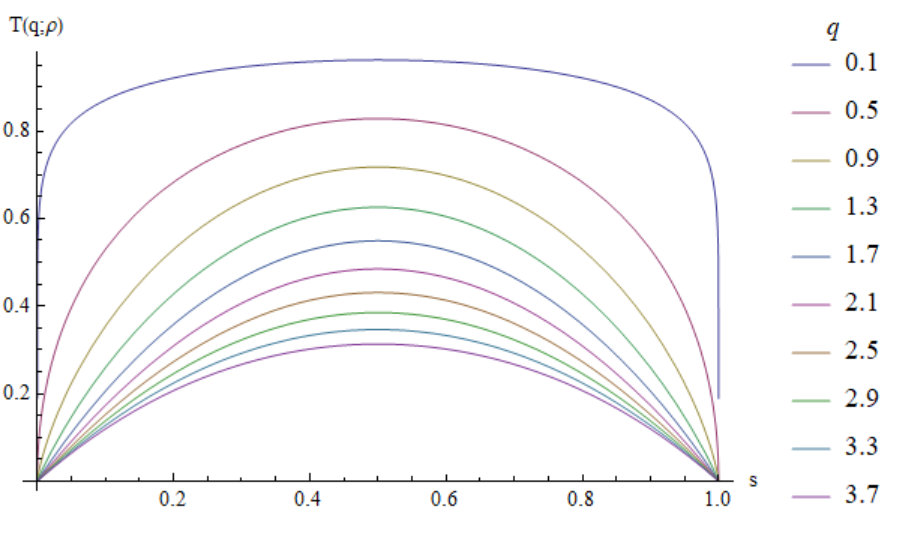
\includegraphics[scale=0.45]{figures/tsallis_ent_plot.png}
\end{center}
for $s=0.5$ Tsallis entropy is not independent of q.
\end{scriptsize}
\end{frame}

\begin{frame}{Example-V(Maximally mixed in N dimensions)}
For
$$ \rho = \sum_{i=0}^{N-1}\rho_{i}\ket{i}\bra{i} = \diag (\rho_{0},\rho_{1},..,\rho_{N-2},\rho_{N-1})=I_{N}/N$$
von Neumann, Renyi case:
\begin{equation}
S(\rho)=R(\alpha;\rho)=\log N
\end{equation}
Tsallis case:
\begin{equation}
T(q;\rho)=\frac{1-N^{1-q}}{q-1}
\end{equation}
\end{frame}

\begin{frame}{Example-III(Werner states)}
\begin{scriptsize}
$$
R(B|A)_{W}=
\frac{\log \left(2^{1-\alpha }\right)-\log \left(4^{-\alpha } \left(3 (1-s)^{\alpha }+(3 s+1)^{\alpha }\right)\right)}{\alpha -1}
$$
\begin{center}
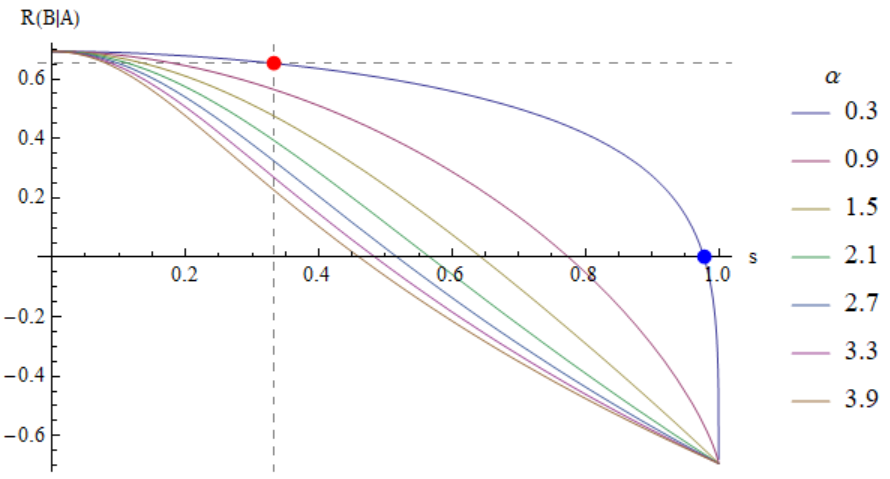
\includegraphics[scale=0.5]{figures/conditional_renyi_werner.png}
\end{center}
As an example, blue point $B$ has the coordinates $(0,0.978043)$ and the red point $R(1/3,0.65241)$ which was found via numerical methods.
\end{scriptsize}
\end{frame}

\begin{frame}{Example-III(Werner states)}
\begin{scriptsize}
$$
T(B|A)_{W}= \frac{2^{-q-1} \left(-3 (1-s)^q-(3 s+1)^q+2^{q+1}\right)}{q-1}
$$
\begin{center}
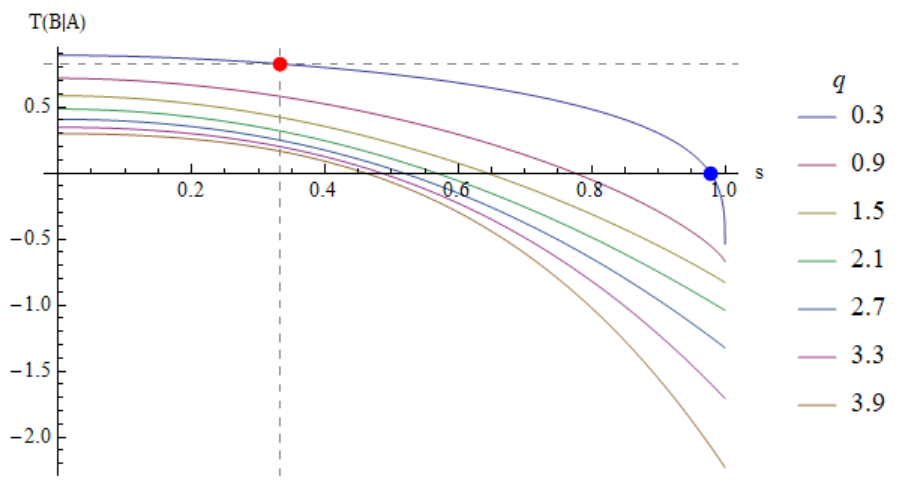
\includegraphics[scale=0.5]{figures/conditional_tsallis_werner.png}
\end{center}
Blue point $B(0,0.978043)$ and the red point $R(1/3,0.826907)$.
\end{scriptsize}
\end{frame}

\subsection{Quantum Relative entropy}
\begin{frame}{Theory}
\begin{tiny}
\begin{definition}(Quantum Relative Entropy) The quantum relative entropy $D(\rho \| \sigma)$ between density operators $\rho \in \mathcal{D}(\mathcal{H})$ and $\sigma \in \mathcal{L}(\mathcal{H})$ is defined by:
\begin{equation*}
D(\rho \| \sigma)= 
 \begin{cases} 
      \operatorname{Tr}[ \rho\log \rho ]-\operatorname{Tr} [ \rho \log \sigma]   & \operatorname{supp}(\rho) \subseteq \operatorname{supp}(\sigma) \\
      \infty & otherwise 
\end{cases}
\end{equation*}
\end{definition}
\begin{alertblock}{Note}
The quantum relative entropy is 0 iff $\rho = \sigma$.
\end{alertblock}
\begin{definition}(Heuristic Quantum Relative Entropy)The heuristic quantum relative entropy $Q(\rho \| \sigma)$ between the $d \times d$ density matrices $\rho$ and $\sigma$ is defined by:
\begin{equation*}
Q(\rho \| \sigma)= S(\rho)-\lim_{\epsilon \to -\infty} \big( \operatorname{Tr}[\rho  G(\epsilon; \sigma)] \big)
\end{equation*}
in which $G: [0,1] \rightarrow \mathbb{R}$ as:
\begin{equation*}
G(\epsilon;x)=
\begin{cases}
   \ln x   &   x \in (0,1] \\
   \epsilon  &   x=0
\end{cases}
\end{equation*}
$\epsilon$ is a free parameter with $\epsilon \in \bbR$.
\end{definition}
\end{tiny}
\end{frame}

\begin{frame}{Example-VI($\small \sigma_u=\ket{\psi(u)}\bra{\psi(u)}$ vs $\sigma_v=\ket{\psi(v)}\bra{\psi(v)}$)}
\begin{scriptsize}
\begin{align*}
&Q(\sigma_u \| \sigma_v) = \\
&S(\sigma_u)-\lim_{\epsilon \to -\infty} \left\{ \Tr \left[
\sigma_u M_v
\left(
\begin{array}{cccc}
 G(\epsilon;1) & 0 & 0 & 0 \\
 0 &  G(\epsilon;0) & 0 & 0 \\
 0 & 0 &  G(\epsilon;0) & 0 \\
 0 & 0 & 0 &  G(\epsilon;0) \\
\end{array}
\right) M_v^{-1} \right] \right\} \nonumber \\[0.5em]
&= -\lim_{\epsilon \to -\infty} \left\{ \Tr \left[ \sigma_u
\left(
\begin{array}{cccc}
 \epsilon  \sin ^2(v) & 0 & 0 & -\epsilon  \cos (v) \sin (v) \\
 0 & \epsilon  & 0 & 0 \\
 0 & 0 & \epsilon  & 0 \\
 -\epsilon  \cos (v) \sin (v) & 0 & 0 & \epsilon  \cos ^2(v) \\
\end{array}
\right)
 \right] \right\} \nonumber \\[0.5em]
&=-\lim_{\epsilon \to -\infty} \left( \epsilon  \sin ^2(v-u) \right) \nonumber \\[0.5em]
&=
\begin{cases}
   +\infty   &   u \neq v\\
   0  &   u=v
\end{cases}
\end{align*}
This result is expected. Different pure states diverge while the quantum relative entropy is zero if the matrix arguments are identical.
\end{scriptsize}
\end{frame}

\begin{frame}{Example-VII($\sigma(\theta)$ vs W)}
\begin{scriptsize}
\begin{equation*}
Q(\sigma\|W)=\frac{1}{2} \left(\log \left(\frac{16}{-3 s^2+2 s+1}\right)+\sin (2 \theta ) \log \left(\frac{1-s}{3 s+1}\right)\right)
\end{equation*}
\begin{center}
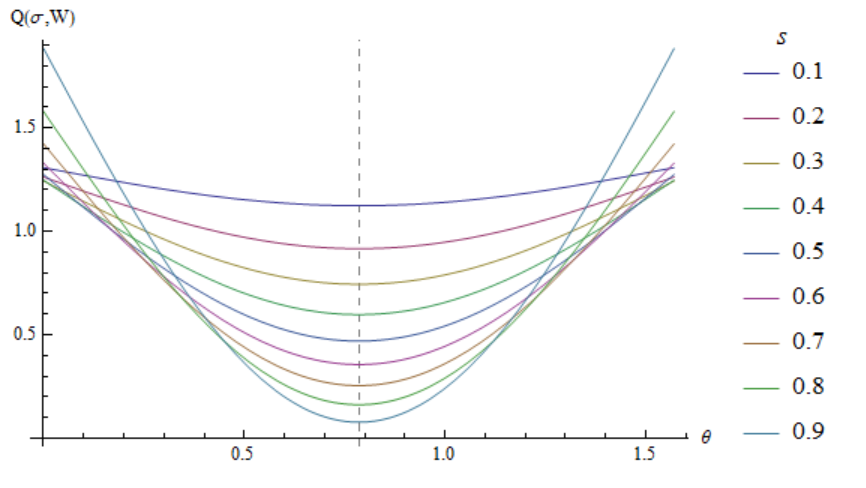
\includegraphics[scale=0.5]{figures/PureMixedRelativeEntropy.png}\label{fig5}
\end{center}
As we can see this measure of departure can detect the maximum entanglement of state $\sigma(\theta)$. We can easily check that $Q(W\|\sigma)$ diverges.
\end{scriptsize}
\end{frame}

\section{Conclusions}
\begin{frame}{Conclusions}
\begin{scriptsize}
\begin{itemize}
\item It is tempting to conjecture that if there can be designed an experiment that measures $Q(\sigma\|W)$ directly, we can detect and quantify the entanglement of the pure state $\sigma(\theta)$.
\item It is proven for the quantum relative entropy that:
\begin{equation*}
D(\rho \| \sigma)=\lim _{\varepsilon \to 0^{+}} D(\rho \| \sigma+\varepsilon I)
\end{equation*}
using a different function $G(\varepsilon ;x)=x+\varepsilon$. Since different functions can be used to heuristically determine the quantum relative entropy, questions are raised regarding the class of functions $G(\varepsilon;x)$.
\item Figures in slide \ref{fig1},\ref{fig5} examples II,VI,VII do not exist in the current literature. 
\end{itemize}
\end{scriptsize}
\end{frame}
\end{document}
